\apendice{Especificación de diseño}

\section{Introducción}
En esta sección se detallan los aspectos más importantes de la aplicación: los datos utilizados, los procedimientos de la aplicación, la arquitectura de la aplicación y el diseño de las interfaces.

\section{Diseño de datos}

\section{Diseño procedimental}

\section{Diseño arquitectónico}

\section{Diseño de interfaces}
En este apartado, se muestran los diseños realizados de la aplicación web con la función de mostrar las funcionalidades que tendría la aplicación web, además de mostrar una interfaz con aspecto amigable.

\subsection{Vista de usuario}
Se muestra el diseño de las interfaces para un usuario sin privilegios. Las figuras \ref{fig:inicio_de_sesion}, \ref{fig:inicio}, \ref{fig:inicio_1} y \ref{fig:resultado} son las correspondientes a este apartado.
\begin{figure}[h]
	\frame{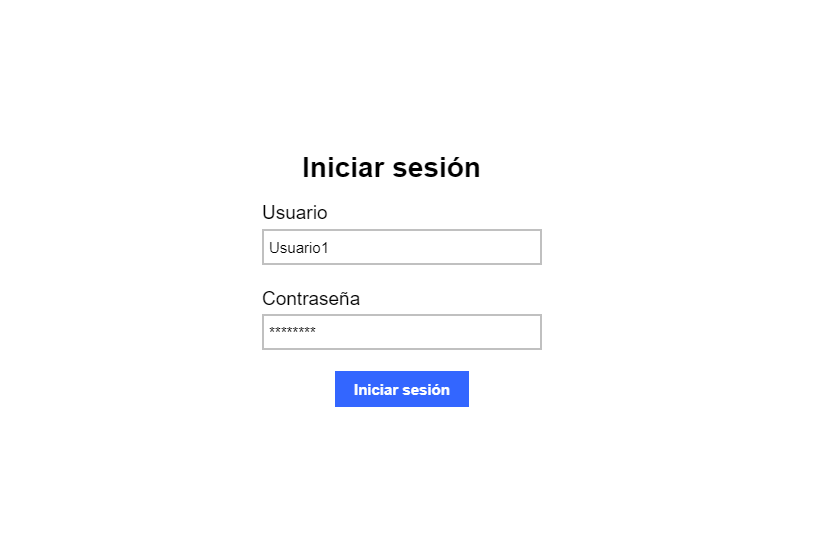
\includegraphics[width=1\textwidth]{inicio_de_sesion}}
	\caption{Pantalla de inicio de sesión de un usuario.}
	\label{fig:inicio_de_sesion}
\end{figure}

\begin{figure}[h]
	\frame{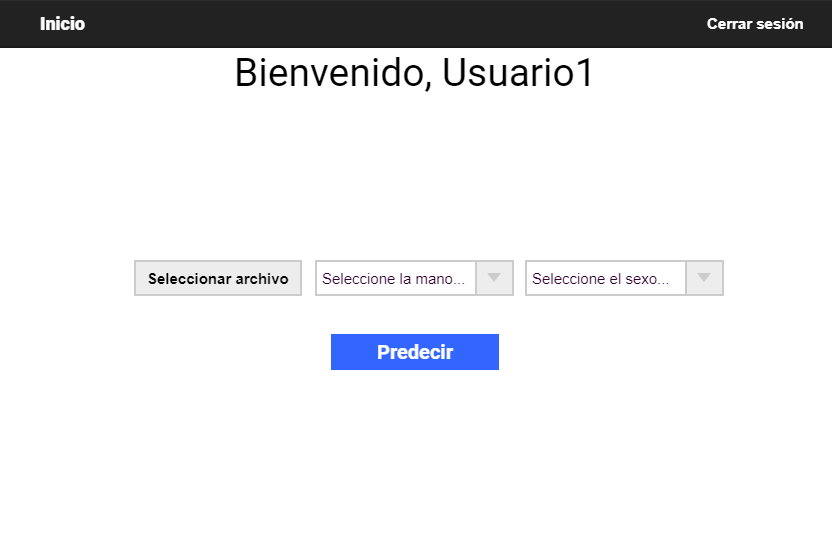
\includegraphics[width=1\textwidth]{inicio}}
	\caption{Pantalla inicial de un usuario.}
	\label{fig:inicio}
\end{figure}

\begin{figure}[h]
	\frame{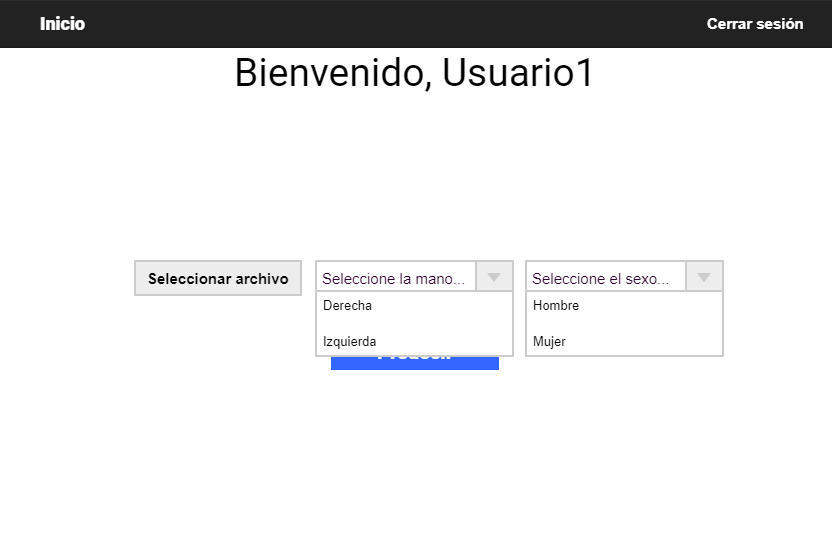
\includegraphics[width=1\textwidth]{inicio_1}}
	\caption{Pantalla inicial de un usuario con las listas desplegadas.}
	\label{fig:inicio_1}
\end{figure}

\begin{figure}[h]
	\frame{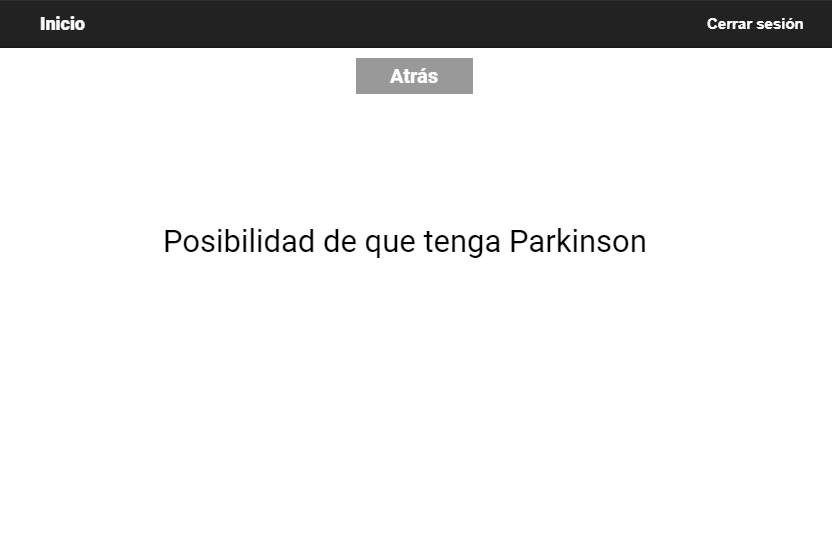
\includegraphics[width=1\textwidth]{resultado}}
	\caption{Pantalla con el resultado de la predicción de un usuario.}
	\label{fig:resultado}
\end{figure}

\subsection{Vista de administrador}
Se muestra el diseño de las interfaces para un usuario con privilegios. Las figuras \ref{fig:inicio_de_sesion_admin}, \ref{fig:inicio_admin}, \ref{fig:inicio_1_admin}, \ref{fig:resultado_admin}, \ref{fig:gestionar_usuarios}, \ref{fig:agregar_usuario}, \ref{fig:modificar_usuario}, \ref{fig:eliminar_usuario} y \ref{fig:modificar_modelo} son las correspondientes a este apartado.
\begin{figure}[h]
	\frame{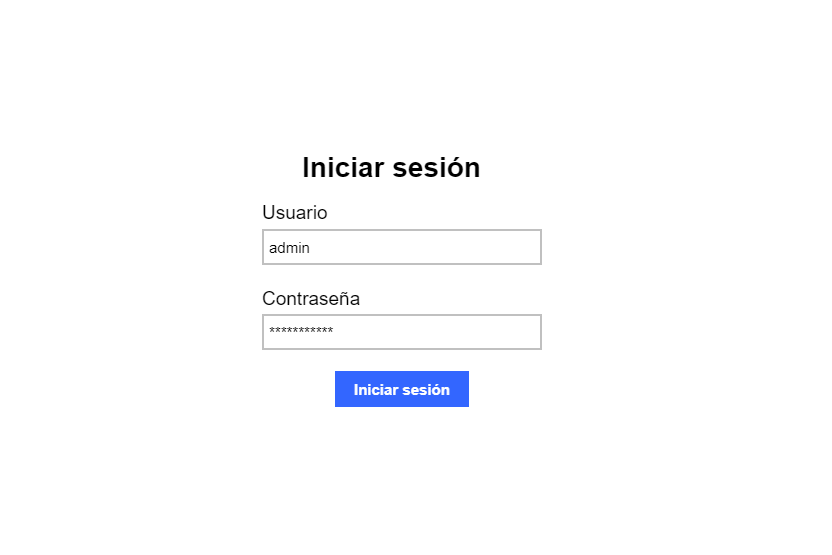
\includegraphics[width=1\textwidth]{inicio_de_sesion_admin}}
	\caption{Pantalla de inicio de sesión de un usuario administrador.}
	\label{fig:inicio_de_sesion_admin}
\end{figure}

\begin{figure}[h]
	\frame{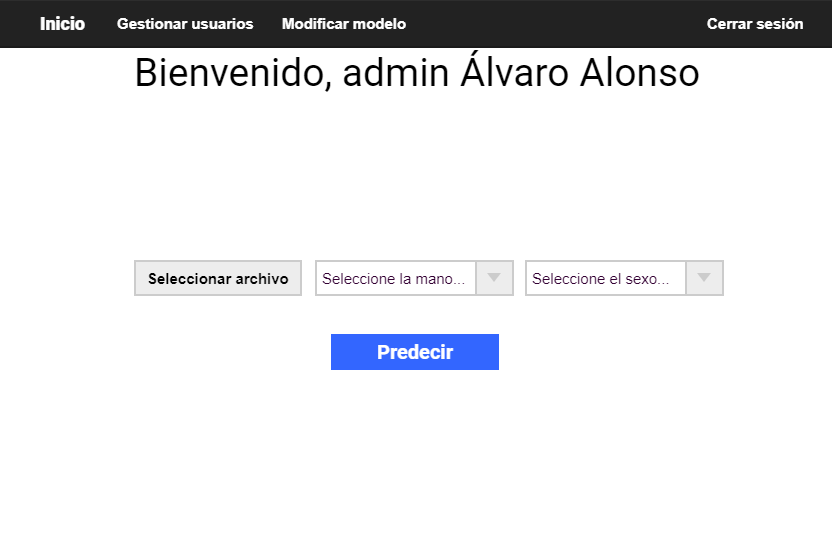
\includegraphics[width=1\textwidth]{inicio_admin}}
	\caption{Pantalla inicial de un usuario administrador.}
	\label{fig:inicio_admin}
\end{figure}

\begin{figure}[h]
	\frame{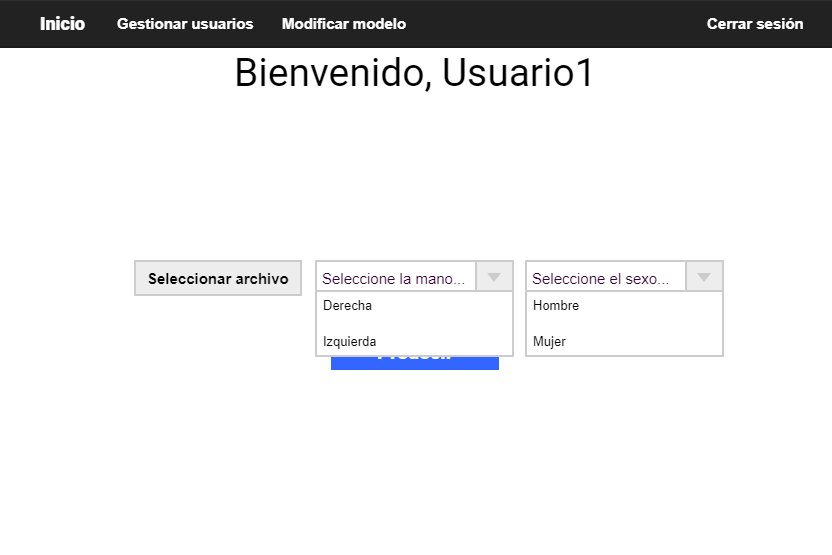
\includegraphics[width=1\textwidth]{inicio_admin_1}}
	\caption{Pantalla inicial de un usuario administrador con las listas desplegadas.}
	\label{fig:inicio_1_admin}
\end{figure}

\begin{figure}[h]
	\frame{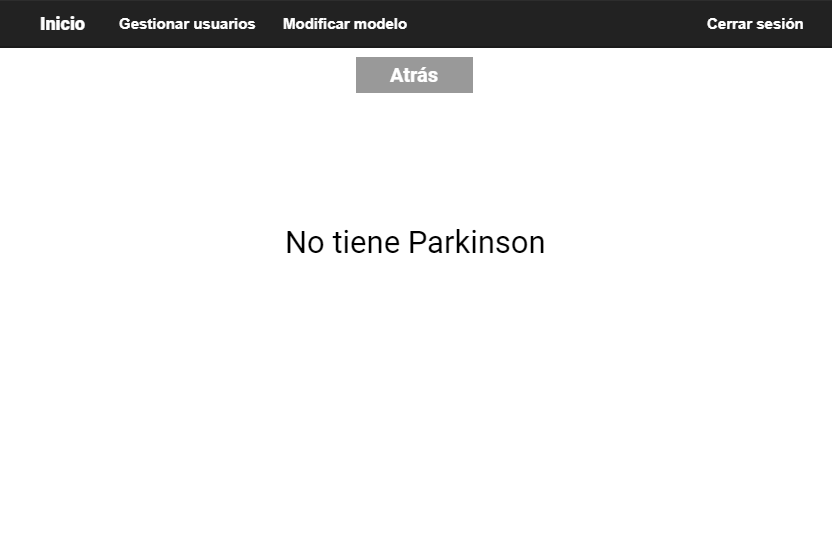
\includegraphics[width=1\textwidth]{resultado_admin}}
	\caption{Pantalla con el resultado de la predicción de un usuario administrador.}
	\label{fig:resultado_admin}
\end{figure}

\begin{figure}[h]
	\frame{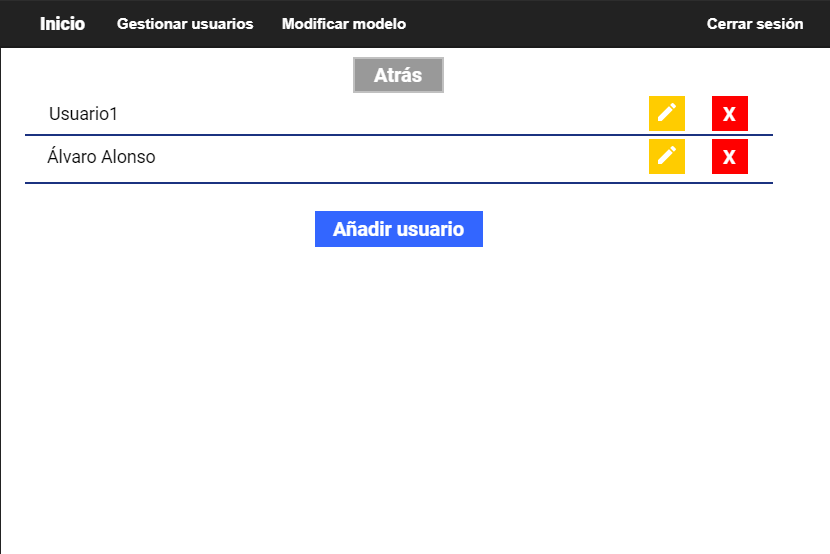
\includegraphics[width=1\textwidth]{gestionar_usuarios}}
	\caption{Pantalla con el listado de los usuarios dados de alta en la aplicación.}
	\label{fig:gestionar_usuarios}
\end{figure}

\begin{figure}[h]
	\frame{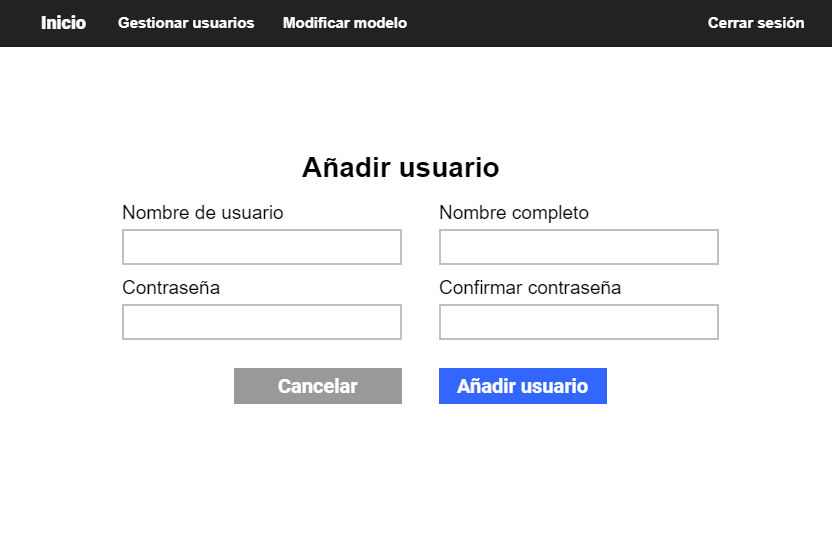
\includegraphics[width=1\textwidth]{agregar_usuario}}
	\caption{Pantalla con el formulario para dar de alta a un usuario.}
	\label{fig:agregar_usuario}
\end{figure}

\begin{figure}[h]
	\frame{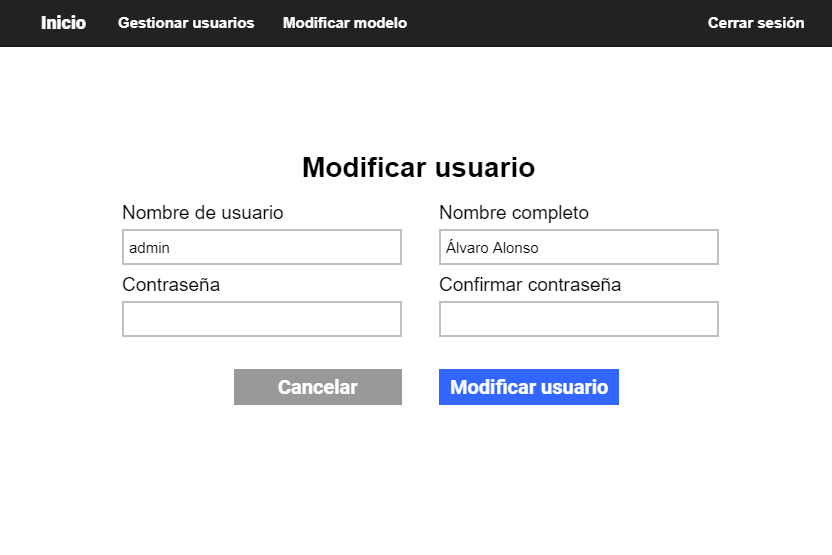
\includegraphics[width=1\textwidth]{modificar_usuario}}
	\caption{Pantalla con el formulario para modificar un usuario existente.}
	\label{fig:modificar_usuario}
\end{figure}

\begin{figure}[h]
	\frame{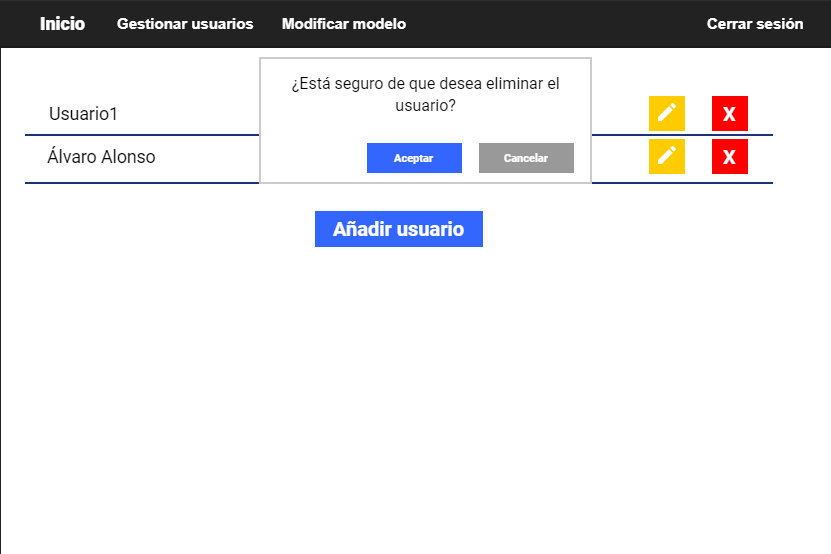
\includegraphics[width=1\textwidth]{eliminar_usuario}}
	\caption{Pantalla con la confirmación para borrar el usuario.}
	\label{fig:eliminar_usuario}
\end{figure}

\begin{figure}[h]
	\frame{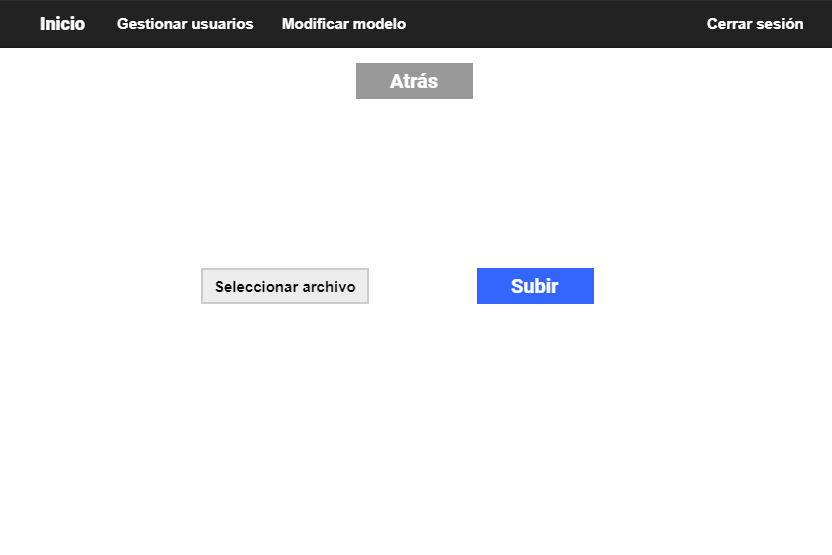
\includegraphics[width=1\textwidth]{modificar_modelo}}
	\caption{Pantalla con la subida del modelo al servidor.}
	\label{fig:modificar_modelo}
\end{figure}
